%%%%%%%%%%%%%%%%%%%%%%%%%%%%%%%%%%%%%%%%%%%%%%%%%
\section[Triangulation]{Triangulation}
%------------------------------------------------
\begin{frame}
\frametitle{Triangulation}
\note{la dernière étape consiste à effectuer une triangulation des points}
\centering
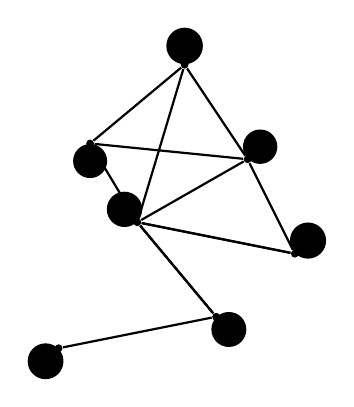
\begin{tikzpicture}[scale=2, every node/.style={circle, fill=black, inner sep=1pt}]
  % Points
  \node (A) at (0,0) {};
  \node (B) at (1,0.2) {};
  \node (C) at (0.5,0.8) {};
  \node (D) at (1.5,0.6) {};
  \node (E) at (1.2,1.2) {};
  \node (F) at (0.2,1.3) {};
  \node (G) at (0.8,1.8) {};

  % Triangles
  \draw[thick] (A) -- (B) -- (C) -- cycle;
  \draw[thick] (B) -- (C) -- (D) -- cycle;
  \draw[thick] (C) -- (D) -- (E) -- cycle;
  \draw[thick] (C) -- (E) -- (F) -- cycle;
  \draw[thick] (C) -- (F) -- (G) -- cycle;
  \draw[thick] (C) -- (G) -- (E) -- cycle;

  % Optional: labels
  \node[anchor=north east] at (A) {A};
  \node[anchor=north west] at (B) {B};
  \node[anchor=south east] at (C) {C};
  \node[anchor=south west] at (D) {D};
  \node[anchor=south west] at (E) {E};
  \node[anchor=north] at (F) {F};
  \node[anchor=south] at (G) {G};
\end{tikzpicture}

\vspace{0.5em}
\textit{Exemple de triangulation d’un ensemble de points en 2D.}
\end{frame}


